\documentclass{article}

\usepackage{graphicx}
\usepackage{tikz}
\usepackage{tikzsymbols}
\usetikzlibrary{calc,patterns,shapes.geometric}
\pagestyle{empty}
\usepackage[margin=0pt]{geometry}
\geometry{papersize={14in,12in}}

\def\centerarc[#1](#2)(#3:#4:#5){\draw[#1] ($(#2)+({#5*cos(#3)},{#5*sin(#3)})$) arc (#3:#4:#5);}

\begin{document}
	\begin{figure}
		\centering
		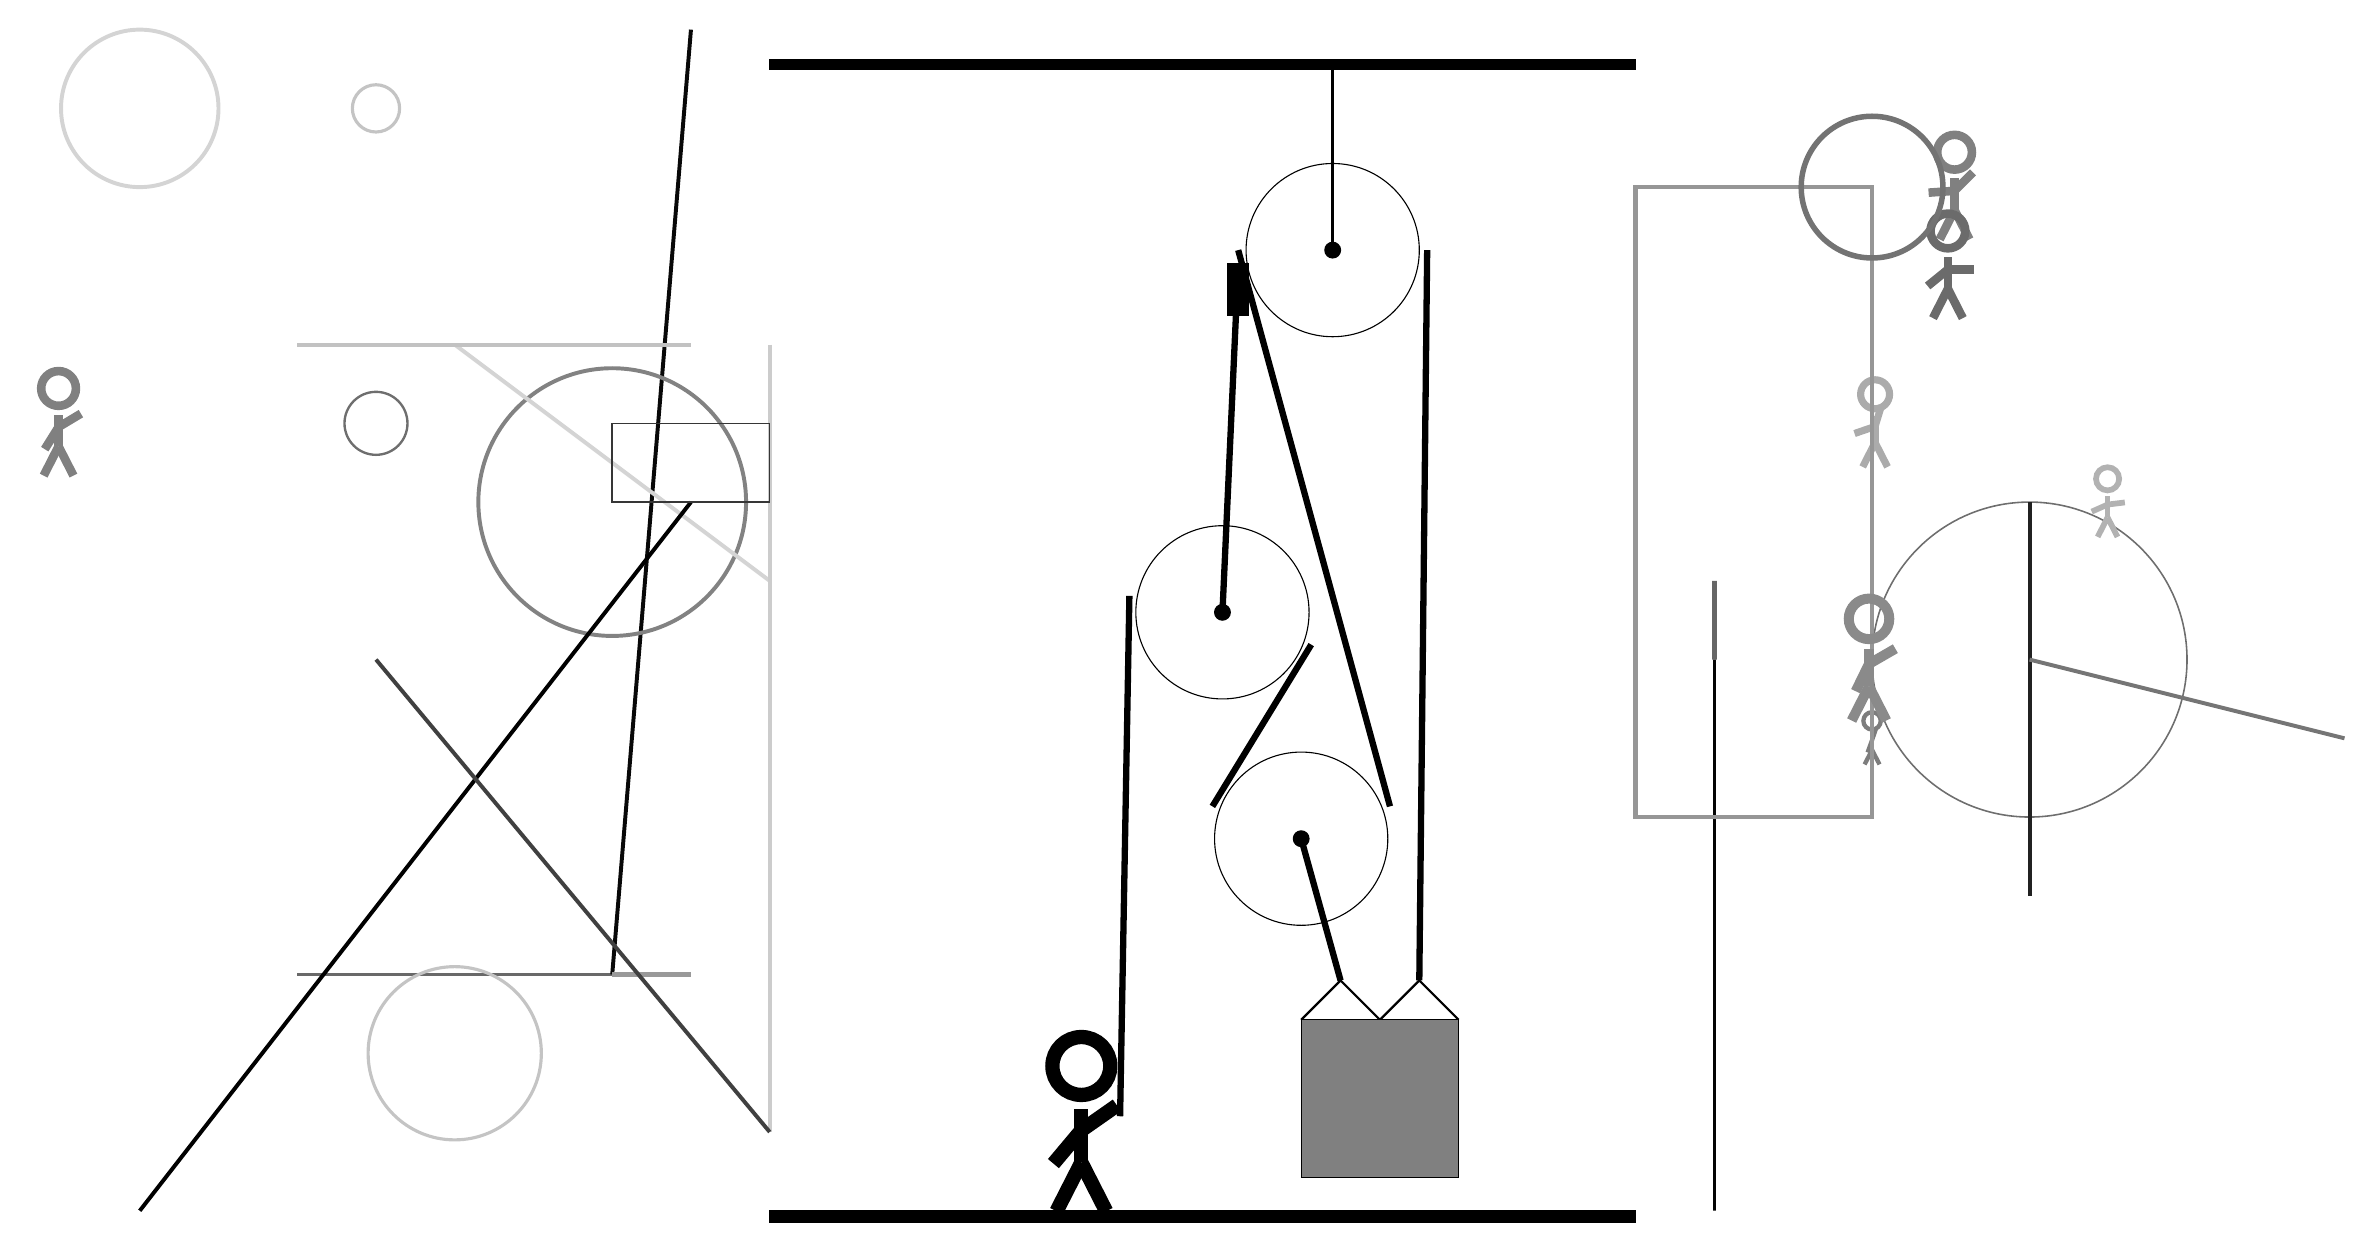
\begin{tikzpicture}
			%%%%% START %%%%%
			
			\draw[fill=black] (-6, 11.5) rectangle (5, 11.625);
			
			\draw (-0.25, 4.6) circle (1.1);
			\draw[fill=black] (-0.25, 4.6) circle (0.1);
			
			\draw (0.75, 1.725) circle (1.1);
			\draw[fill=black] (0.75, 1.725) circle (0.1);
			
			\draw (1.15, 9.2) circle (1.1);
			\draw[fill=black] (1.15, 9.2) circle (0.1);
			\draw[very thick] (1.15, 9.2) -- (1.15, 11.5);
			
			\draw[thick]  (0.75, -0.575) -- (1.25, -0.075) -- (1.75, -0.575) -- (2.25, -0.075) -- (2.75, -0.575);
			\draw[fill=black!50] (0.75, -0.575) rectangle (2.75, -2.575);
			
			\draw[line width=0.5mm, color=black!59](-8, 0) -- (-12, 0);
			
			\node[line width=0.4mm, color=black!50] at (-15, 7) {\Strichmaxerl[6][58][31]};
			\draw[line width=0.5mm, color=black!97](-8, 0) -- (-7, 12);
			\draw [line width=0.5mm, color=black!49](-8, 6) circle (1.7);
			\node[line width=0.7mm, color=black!50] at (9, 10) {\Strichmaxerl[6][4][45]};
			\draw[line width=0.7mm, color=black!60] (6, 4) rectangle (6, 5);
			\draw[line width=0.3mm, color=black!99] (6, -3) rectangle (6, 4);
			\node[line width=0.7mm, color=black!58] at (9, 9) {\Strichmaxerl[6][39][0]};
			\draw[line width=0.5mm, color=black!17](-10, 8) -- (-6, 5);
			\draw [line width=0.2mm, color=black!57](10, 4) circle (2.0);
			
			\draw[line width=0.5mm, color=black!20](-6, 8) -- (-6, -2);
			\draw[line width=0.5mm, color=black!24](-7, 8) -- (-12, 8);
			\node[line width=0.5mm, color=black!51] at (8, 3) {\Strichmaxerl[3][70][71]};
			\draw[line width=0.6mm, color=black!40] (-7, 0) rectangle (-8, 0);
			\draw[line width=0.5mm, color=black!87](10, 6) -- (10, 1);
			\draw [line width=0.3mm, color=black!57](-11, 7) circle (0.4);
			
			\node[line width=0.6mm, color=black!33] at (8, 7) {\Strichmaxerl[5][19][73]};
			\draw[line width=0.6mm, color=black!41] (5, 2) rectangle (8, 10);
			\node[line width=0.6mm, color=black!30] at (11, 6) {\Strichmaxerl[4][24][7]};
			
			\draw[line width=0.5mm, color=black!54](10, 4) -- (14, 3);
			\draw [line width=0.5mm, color=black!17](-14, 11) circle (1.0);
			\draw [line width=0.7mm, color=black!55](8, 10) circle (0.9);
			
			\draw[line width=0.5mm, color=black!100](-7, 6) -- (-14, -3);
			\node[line width=0.7mm, color=black!46] at (8, 4) {\Strichmaxerl[7][64][30]};
			\draw [line width=0.4mm, color=black!23](-10, -1) circle (1.1);
			
			\draw[line width=0.2mm, color=black!79] (-8, 7) rectangle (-6, 6);
			\draw [line width=0.4mm, color=black!23](-11, 11) circle (0.3);
			\draw[line width=0.5mm, color=black!75](-6, -2) -- (-11, 4);
			
			
			\draw[line width=0.8mm] (-0.25, 4.6) -- (-0.05, 9.0);
			\draw[line width=0.8mm, fill=black](-0.15, 8.4) rectangle (0.05, 9.0);
			\draw[line width=0.8mm] (-1.55, -1.8) -- (-1.4318, 4.8083);
			\centerarc[line width=0.8mm](-0.25, 4.6)(-20:170:1.2000000000000002);
			\draw[line width=0.8mm] (0.8776, 4.1896) -- (-0.3776, 2.1354);
			\centerarc[line width=0.8mm](0.75, 1.725)(160:380:1.2000000000000002);
			\draw[line width=0.8mm] (1.8776, 2.1354) -- (-0.05, 9.2);
			\draw[line width=0.8mm](0.75, 1.725) -- (1.25, -0.075);
			\centerarc[line width=0.8mm](1.15, 9.2)(0:180:1.2000000000000002);
			\draw[line width=0.8mm] (2.35, 9.2) -- (2.25, -0.075);
			
			\node at (-2, -1.9) {\Strichmaxerl[10][50][35]};
			
			\draw[fill=black] (-6, -3) rectangle (5, -3.15);
			
			%%%%% END %%%%%
		\end{tikzpicture}
	\end{figure}	
\end{document}